% +--------------------------------------------------------------------+
% | Appendix B Page (Optional)                                         |
% +--------------------------------------------------------------------+

\cleardoublepage

\chapter{Calidad del código}
\label{Appendix:Key2}

Una vez acabado el código del proyecto, decidimos certificar su calidad mediante \href{https://www.codacy.com}{Codacy}.
Codacy es una herramienta que proporciona nuestro controlador de versiones GitHub. Sencillamente revisa todas y cada una de las líneas del código, para hacerlo más sencillo, escalable y seguro. Genera un informe con los errores y te dice qué grado de calidad tiene, siendo A el más alto. (\cite{ARP:Codacy:2017})

\begin{figure}[htb]
	\begin{center}
		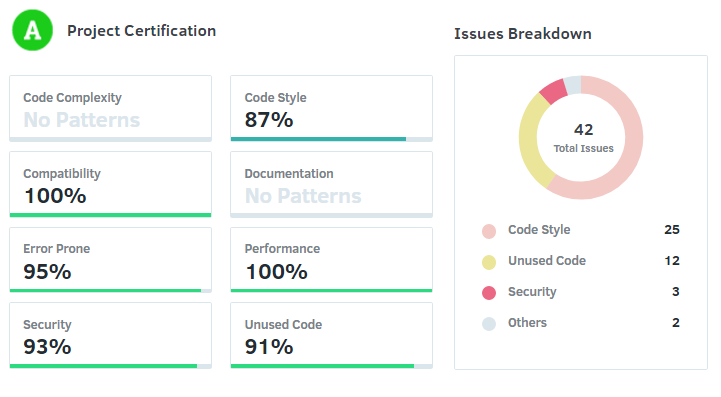
\includegraphics[height=3.5in]{figures/codacy.png}
		\caption{Informe de nuestro proyecto [Fuente: \href{https://www.codacy.com}{Codacy}] \label{codacy}}
	\end{center}
\end{figure}
